\chapter{Description of the situation (rich picture and forbilleder)}\fxnote{Dette chapter skal måske rykkes. Kan vi følge SU struktur fra slides!!!!!!!}

\section{Rich Picture}
Figure \ref{RigtBillede} shows a Rich picture. This rich picture gives an overview of the users situation from the viewers position. The symbols represent different units, processes and problems. To begin with we will look at the symbols and explain them. Afterwards the situation will be explained in depth.

  \begin{figure}[H]
	\centering
	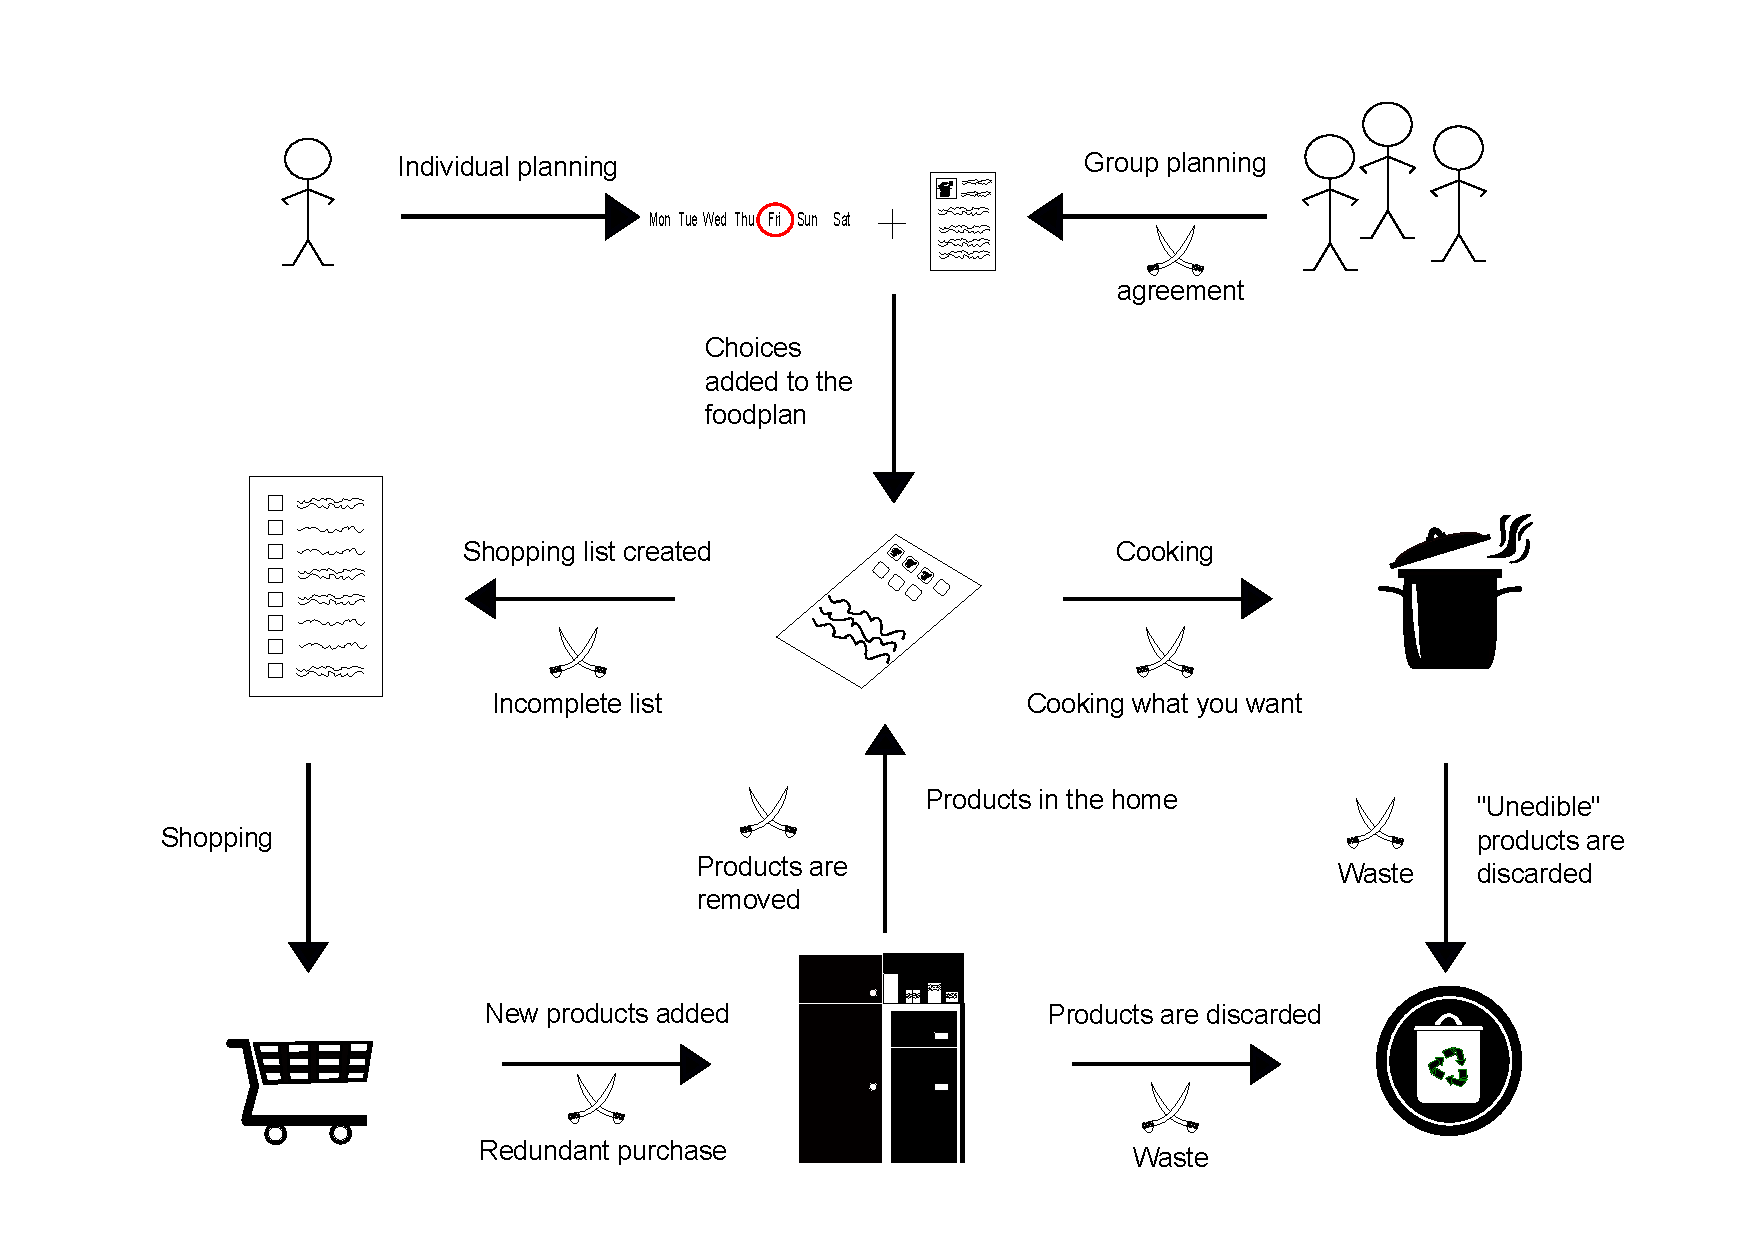
\includegraphics[width=1.00\textwidth]{Grafik/FoodPlanner/InkscapeTegninger/RigtBillede.pdf}
	\caption{A rich picture of the user's situation from the viewers position}
	\label{RigtBillede}
\end{figure}
\fxnote{resize elementer så der er lige store + kosmetiske fejl}
\textbf{Units} includes people, physical objects, organizations and roles. On the top line there are the stick man symbol which is used to represent a user and to the top right there are the group of users symbol. On the middle line there the overview of the food plan symbol and shopping list symbol which is used to depict the user's overview of the two units. On the bottom line there are the inventory symbol used to depict the household's storage of food products and the trashcan symbol.    

\textbf{Processes} includes different categories such as work and production, planning and control and information treatment. In Figure \ref{RigtBillede} All of the arrows between the symbols signifies different processes. On the top line there are two arrows pointing into the scheduled meal symbol signifying the process of choosing a specific day and a associated recipe. The choice is then added to the food plan showed by the vertical arrow pointing down to the overview of the food plan symbol. ON the middle line there are two horizontal arrows. The arrow pointing to the left shows how a shopping list is created using data from the food plan. The arrow pointing to the right signifies the cooking work process. Below the middle line there are three vertical arrows. The arrow on the left pointing downwards shows the shopping process, the middle arrow pointing upwards signifies that the food plan is affected by what products that are in storage and the right arrow pointing downwards shows that products can be discarded when the user is cooking. On the bottom line there are two arrows pointing to the left. The left arrow signifies that products are added to the inventory after they are bought. The right arrow signifies that products can be discarded from the inventory.            

\textbf{Problems} describes the conflicts, contradictions and discrepancies in the situation. On the top line there are one conflict under the group planning process. This conflict is named synchronizing and happens when multiple users are scheduling meals. On the middle line there a two conflicts. The left one is named incomplete list and happens if the user does not have a complete list over the items that are needed in the food plan. The left conflict is named cooking what you want and describes that users can cook meals that are not on their food plan. Next there are the products removed conflict which happens when a user physically removes a product from the inventory. Next to this conflict we have the waste conflict which happens when food is thrown out during cooking. This conflict can also happen when products from the inventory is discarded as shown on the left side of the bottom line On the bottom line there are two more conflicts. The left one named redundant purchases happens when the user buys larger quantities of food than the shopping list advises.             

\textbf{Situation explained}

Figure \ref{RigtBillede} can also be divided into different context areas. The areas represent contexts in which different symbols are performed most often. The contexts are in the home and out of the home. Some symbols can belong in both contexts such as planning your meals which includes the user symbols, day + recipe and food plan overview symbols.       